\section*{3. Numerisk løsning af systemer af differentialligninger}
% 
%
\begin{color}{AAUblue2}
%
%DEN HER GIDER JEG I HVERT FALDE IKKE OG SKRIVE IND XD SÅÅÅÅ EN ELLER ANDDEN SOM GODT KUNNE LAVE ANDET END AT SPILLE COMPUTERSPIL FÅR ÆREN AF DETTE XD HEHEHEHEHEHEHE
%\\\\
%meh 
%\\\\
RK4 metoden og de andre metoder kan anvendes til numerisk løsning af systemer af differentialligninger. 
Følgende tager udgangspunkt i et konkret eksempel. Der er givet et system af differentialligninger, som anvendes til modellering af en ufarlig infektion i population. 
Populationen består af $N$ individer og antages konstant i tid. Den opdeles i tre kategorier. $x_1(t)$ er antallet af individer
der er modtagelige for smitte på tidspunktet $t$. $x_2(t)$ er antallet af smittede individer.
Disse kan smitte de individer der er modtagelige. 
$x_3(t)$ betegner individer der enten er immune, eller som er blevet immune efter at have været smittet.
%
Modellen er beskrevet ved følgende tre differentialligninger: 
%
\begin{align}
\frac{dx_1}{dt} & = - \alpha x_1 x_2, \\
\frac{dx_2}{dt} & = \alpha x_1 x_2 - \beta x_2 , \\
\frac{dx_3}{dt} & = \beta x_2.
\end{align}
%
Vi kan skrive systemet og begyndelsesbetingelsen på vektorform som
%
\begin{align*}
\frac{d}{dt} 
\begin{bmatrix}
x_1 (t) \\
x_2 (t) 
\end{bmatrix} = 
\begin{bmatrix}
- \alpha x_1 (t) x_2 (t) \\
\alpha x_1 (t) x_2 (t) - \beta x_2 (t) 
\end{bmatrix}
,
\begin{bmatrix}
x_1 (0) \\
x_2 (0) 
\end{bmatrix}
= 
\begin{bmatrix}
x_{10} \\
x_{20}
\end{bmatrix}
\end{align*}
%
Parameteren $\alpha$ beskriver den rate hvormed de modtagelige individer bliver smittet.
Parameteren $\beta$ beskriver den rate hvormed smittede individer overstår infektionen. 
% 
\end{color}
%
\subsection*{(a) }
%
%
\begin{color}{AAUblue2}
%
Implementér Euler metoden og Runge-Kutta RK4 metoden for vektorfunktioner. 
% 
\end{color}
\\\\
% 
Se \textsc{system-example-modi.py}. Implementeringerne er ved
\textbf{\textit{def euler}}, linje $6$, og \textbf{\textit{def RK4}}, linje $21$.
%
\subsection*{(b) }
% 
%
\begin{color}{AAUblue2}
%
fisk
% 
\end{color}
\\\\
% 
%
\subsection*{(c)}
%
\begin{color}{AAUblue2}
%
Modificer \textsc{opg2-system.py} til et system hvor $\gamma$ kan ændres med udgangspunkt i at modelles første ser ud som følgende 
\begin{align}
\frac{dx_1}{dt} &= - \alpha x_1 x_2 - \gamma x_1, \\
\frac{dx_2}{dt} & = \alpha x_1 x_2 - \beta x_2 , \\
\frac{dx_3}{dt} & = \beta x_2 + \gamma x_1.
\end{align}
%
Beskriv hvad der sker med en ændring i gamma.  
%
\end{color}
\\\\
% 
Se \textsc{opg2-system-vaccine.py}.
\\\\
%
Værdien gamma forøger hvor hurtigt befolkningen bliver immun uden at have været smittet. Jo højere værdi af gamma jo hurtigere bliver befolkningen immun, og det maksimale antal der er smittet på en gang falder også. Det kan ses på figurene at hvis gamma ikke er nul så er antallet der bliver inficeret lavere
%
%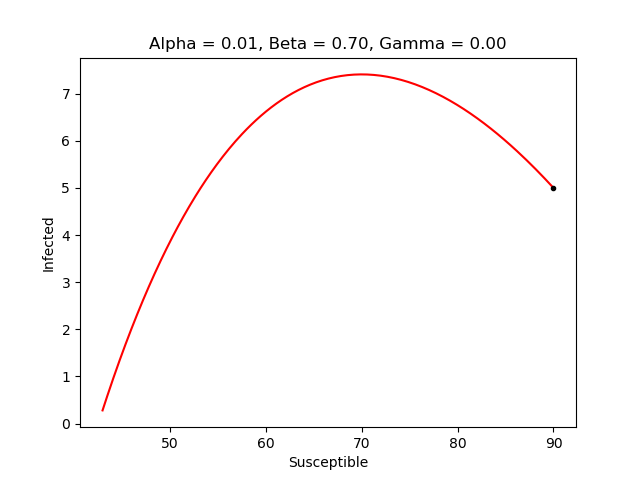
\includegraphics[scale=0.4]{fig/img/a1_b7_g0.png}
%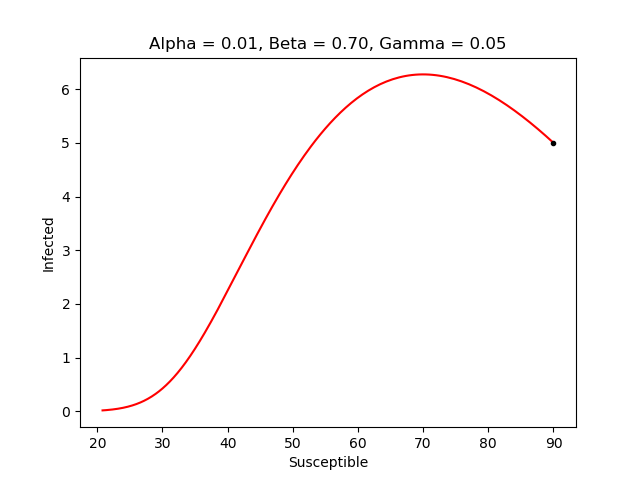
\includegraphics[scale=0.4]{fig/img/a1_b7_g5.png}\\
%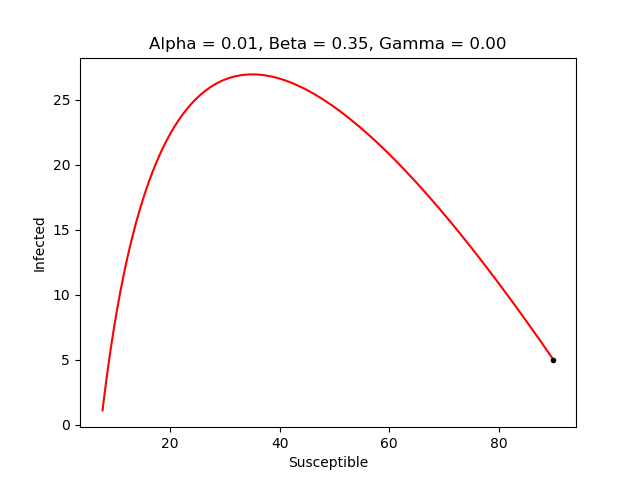
\includegraphics[scale=0.4]{fig/img/a1_b35_g0.png}
%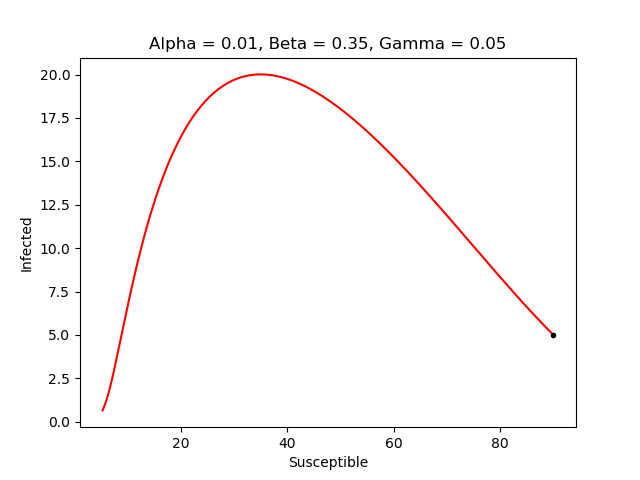
\includegraphics[scale=0.4]{fig/img/a1_b35_g5.png}\\
%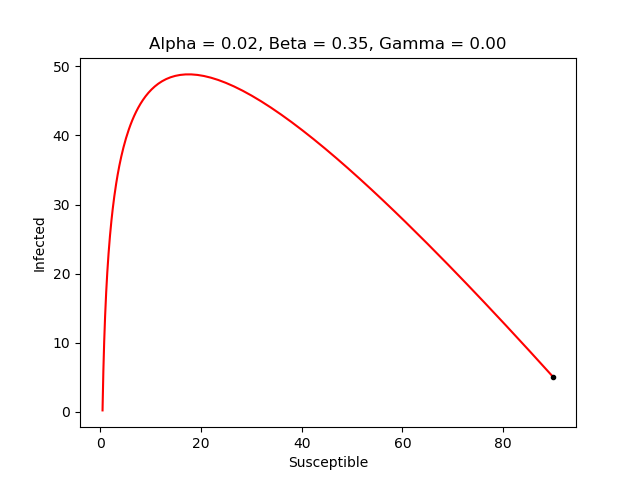
\includegraphics[scale=0.4]{fig/img/a2_b35_g0.png}
%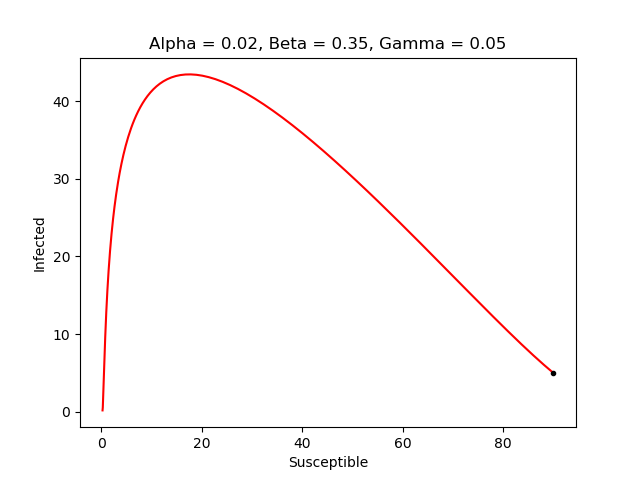
\includegraphics[scale=0.4]{fig/img/a2_b35_g5.png}\\
%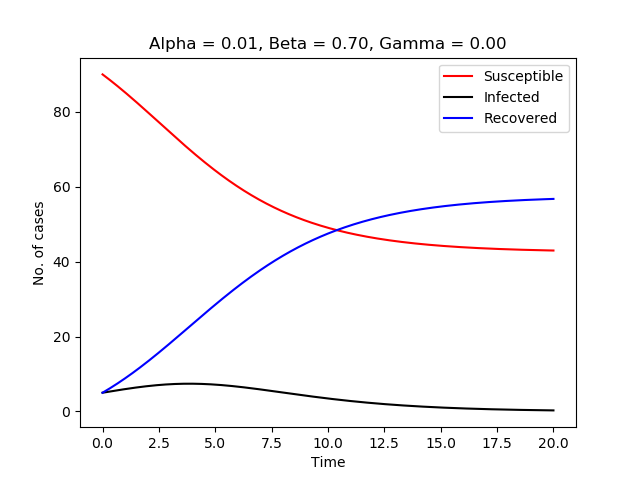
\includegraphics[scale=0.4]{fig/img/t_a1_b7_g0.png}
%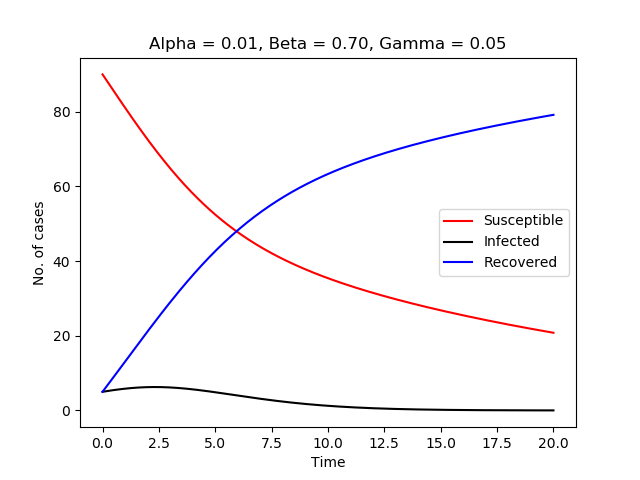
\includegraphics[scale=0.4]{fig/img/t_a1_b7_g5.png}\\
%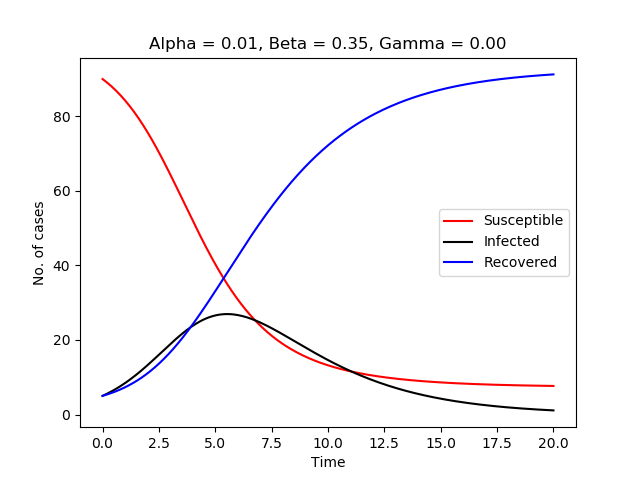
\includegraphics[scale=0.4]{fig/img/t_a1_b35_g0.png}
%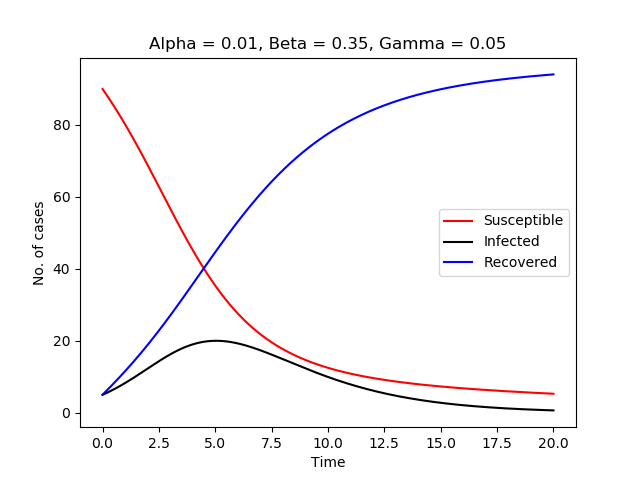
\includegraphics[scale=0.4]{fig/img/t_a1_b35_g5.png}\\
%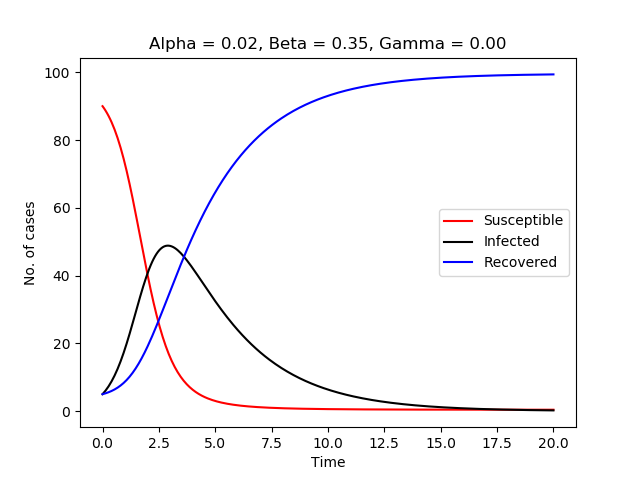
\includegraphics[scale=0.4]{fig/img/t_a2_b35_g0.png}
%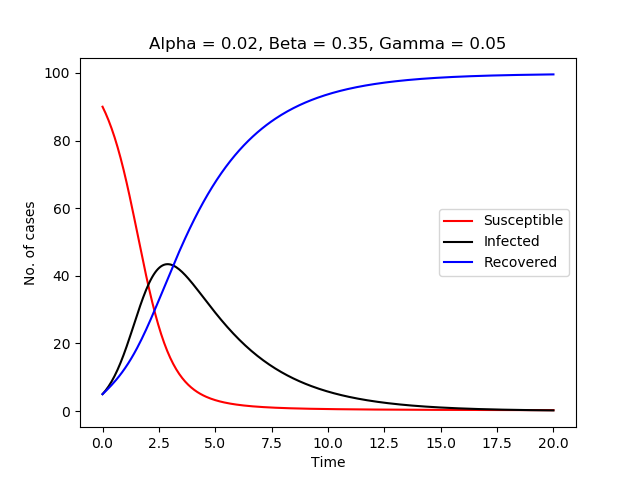
\includegraphics[scale=0.4]{fig/img/t_a2_b35_g5.png}\\
%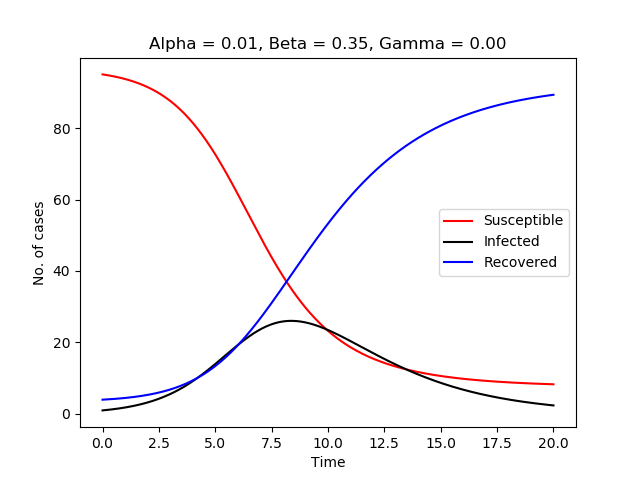
\includegraphics[scale=0.4]{fig/img/t_x1_1_x2_95.png}
%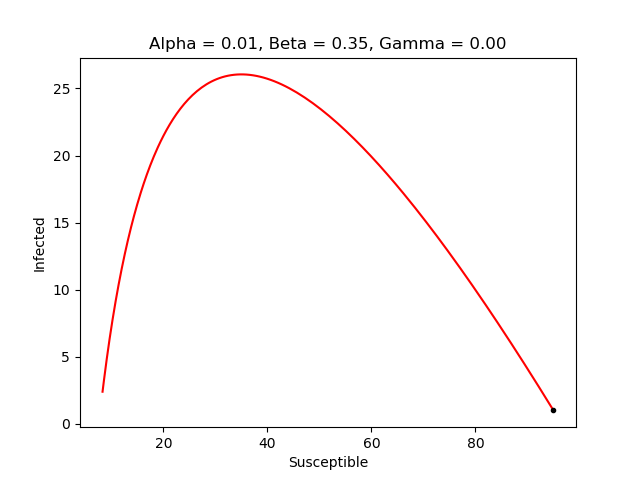
\includegraphics[scale=0.4]{fig/img/x1_1_x2_95.png}\\
\subsection*{(d) }
%
\begin{color}{AAUblue2}
fisk
\end{color}
\\\\
% 
